\section{Number Agreement in Neural Language Models}

\textbf{Will also \emph{gender} agreement results be presented for Italian, as suggested by Fig.~\ref{fig:nounpp}?}

\begin{itemize}
\item Describe previous results: grammatically-controlled sparse
  mechanism for long-range number agreement; refer to results in the
  NACL paper and point to Fig.~\ref{fig:nounpp} below for illustration
    \item Prediction for nested dependencies (Fig.~\ref{fig:design}).
\end{itemize}

\begin{figure*}
    \centering
    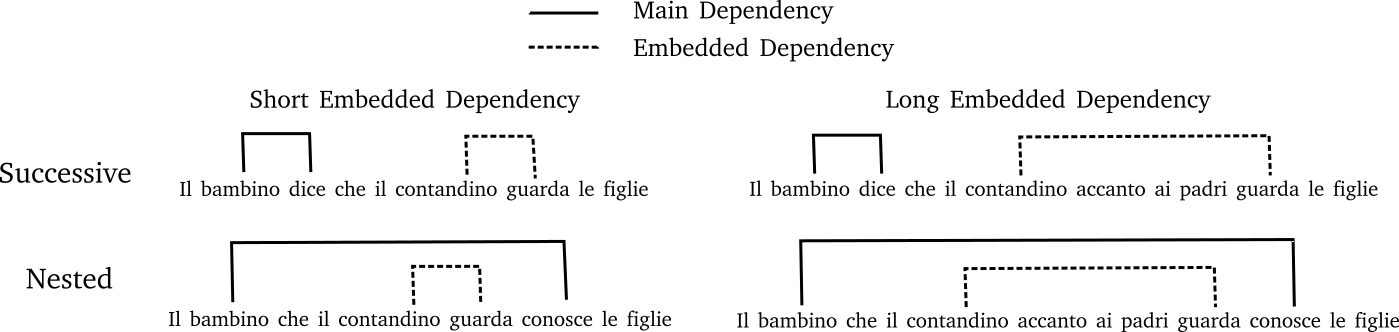
\includegraphics[width=\textwidth]{figures/design.png}
    \caption{\textbf{A full-factorial design for two subject-verb dependencies}. Human subjects and Neural Language Models (NLMs) were presented with sentences from four different syntactic structures, which all have two subject-verb dependencies: a main dependency (continuous lines) and an embedded dependency (dashed). The first factor of the design determines whether the two dependencies are \textit{successive} (top structures) or \textit{nested} (bottom), depending on whether the structure has a sentential complement (SC) or an object-extracted relative clause (objRC), respectively. The second factor determines whether the embedded dependency is \textit{short} (left side) or \textit{long} (right). We refer to the four resulting structures as: SC-short, SC-long, objRC-short and objRC-long.}
    \label{fig:design}
\end{figure*}